\section{Zustandsbasierte Systeme}

\subsection{Finite State Machine (FSM)}
\subsubsection{Asynchrone vs. synchrone FSMs}
\begin{itemize}
  \item Bei (elektronisch implementierten) \textbf{asynchronen} FSMs führen geänderte Inputsignale direkt zu Zustands-\\änderungen. Sie sind deshalb "`schneller"', jedoch äusserst empfindlich auf Glitches und kaum testbar.
  \item Bei \textbf{synchronen} FSMs werden die Inputsignale nur zu diskreten Zeitpunkten betrachtet, diese Systeme sind getaktet.
  \item Softwareimplementationen sind eigentlich immer \textbf{synchron}, da die Rechner getaktet sind. Wenn die Inputsignale mittels Interrupts behandelt werden, ist darauf zu achten, dass die Interrupts nicht fälschlicherweise gesetzt werden (ist Aufgabe der Elektronik)
  \item Rein softwareseitig besteht die Problematik der \textbf{Asynchronizität} nicht
\end{itemize}

\subsubsection{Finite State Machine (FSM)}
\begin{minipage}{0.7\linewidth}
\begin{itemize}
  \item Eine FSM befindet sich immer in einem definierten Zustand
  \item Die Inputs X bezeichnen üblicherweise Ereignisse (\textbf{Events})
  \item Die Outputs Y werden oft auch \textbf{Actions} genannt
  \item Eine FSM benötigt immer Speicherelemente zur Speicherung des \textbf{internen Zustands}
  \item In der Praxis sind zwei FSM-Varianten bekannt: \begin{itemize}
			\item der Mealy-Automat
			\item der Moore-Automat
  			\end{itemize}
\end{itemize}
\end{minipage}%
\begin{minipage}{0.3\linewidth}
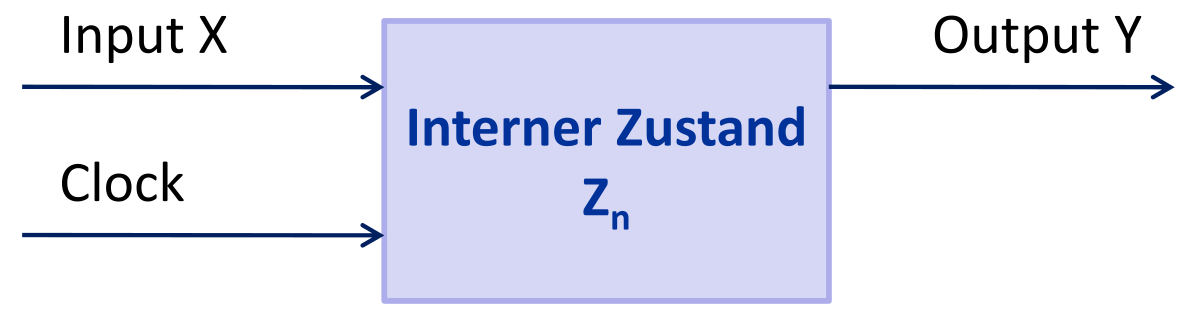
\includegraphics[width=\linewidth]{./images/FSM/fsm}
\vfill\null
\end{minipage}

\subsubsection{Zustands-Ereignis-Diagramm (State-Event-Diagram)}
\begin{itemize}
  \item Die \textbf{Zustände} werden mit einem Kreis gekennzeichnet
  \item Die \textbf{Ereignisse} werden mit Pfeilen zwischen den Zuständen bezeichnet
  (\textbf{Transitionen})
  \item Die \textbf{Aktionen} werden entweder bei den Zuständen geschrieben oder bei den
  Transitionen (je nach Automatentyp)
  \item Die Ausführung einer \textbf{Transition} benötigt keine Zeit. Deshalb sind bei
  der Modellierung oft Zwischenzustände vorzusehen, z.B. "`Closing"', "`Starting
  up"', "`Booting"', etc.
\end{itemize}

\subsubsection{Mealy-Automat}
\begin{itemize}
  	\item Der nächste Zustand $Z_{n+1}$ ist abhängig vom Input X und von $Z_n$:
  	$Z_{n+1}=f(Z_n,X)$
  	\item Der Output Y ist abhängig vom inneren Zustand $Z_n$ \textbf{und vom
 	 Input X}: $Y=g(Z_n, X)$
  	\item Die \textbf{Actions} liegen deshalb bei den \textbf{Transitionen}
\end{itemize}

\subsubsection{Moore-Automat}
\begin{itemize}
	\item Der nächste Zustand $Z_{n+1}$ ist abhängig vom Input X und von $Z_n$:
  	$Z_{n+1}=f(Z_n,X)$
  	\item Der Output Y ist \textbf{nur} abhängig vom inneren Zustand $Z_n$: $Y=g(Z_n)$
  	\item Die \textbf{Actions} liegen deshalb bei den \textbf{Zuständen}
\end{itemize}


\subsubsection{Zustandstabelle}

\renewcommand{\arraystretch}{1}
\begin{tabular}{|l|l|l|l|}
\hline
\textbf{Momentaner Zustand}&\textbf{Ereignis}&\textbf{Nächster
Zustand}&\textbf{Aktionen}\\
\hline
AUS&EIN-Taste&Hochlaufen&Motor ausschalten\\
&&&Kühlung ausschalten\\&&&Grüne Lampe aus\\&&&Rote Lampe aus\\
\hline
Hochlaufen&Drehzahl\_erreicht&Drehzahl\_ok&Motor einschalten\\
&Signal&&Kühlung einschalten\\ \cline{2-3}
&AUS-Taste&AUS&\\\cline{2-3}
&Wasserkühlung&Störung&\\
&Störung&&\\
\hline
Drehzahl\_ok&Wasserkühlung&Störung&Grüne Lampe anzeigen\\
&Störung&&\\ \cline{2-3}
&AUS-Taste&AUS&\\
\hline
Störung&RESET-Taste&AUS&Motor ausschalten\\
&&&Kühlung ausschalten\\&&&Rote Lampe anzeigen\\
\hline
\end{tabular}
\renewcommand{\arraystretch}{1.8}

\subsubsection{Nachteile von Zustandsdiagrammen}
\begin{multicols}{2}
\begin{itemize}
  \item Für einen Resetzustand muss von jedem State zum Resetstate eine Transition gezeichnet werden.
  \item Da Zustandsdiagramme flach sind (es gibt keine Hierarchie), werden sie bei
        praktisch relevanten Aufgaben schnell unübersichtlich
  \item In Zustandsdiagrammen kann keine zeitliche Parallelität modelliert werden
\end{itemize}
\vfill\null
\columnbreak
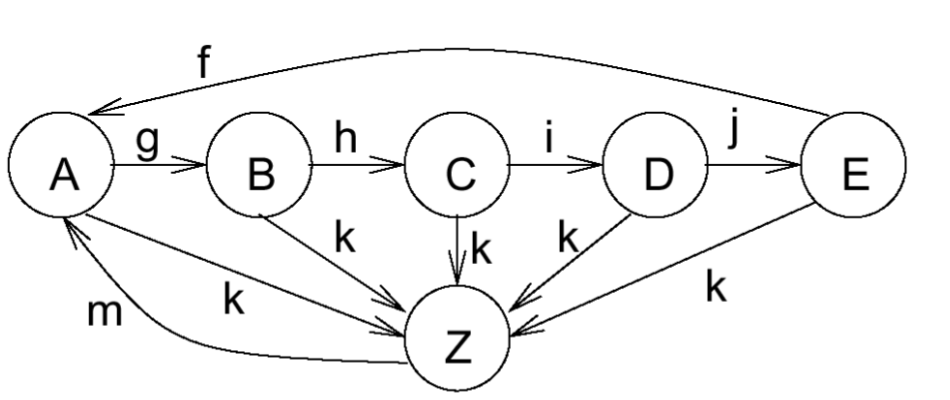
\includegraphics[width=0.9\linewidth]{images/FSM/reset_state}
\end{multicols}

\newcommand{\kreis}[1]{\unitlength1ex\begin{picture}(2.5,2.5)%
\put(0.75,0.75){\circle{3.5}}\put(0.75,0.75){\makebox(0,0){#1}}\end{picture}}

\subsection{Statecharts von Harel}
\subsubsection{Elemente der Statechart}
\begin{tabular}{ll}
$\bullet$&Anfangszustand (initial pseudo state)\\
$\diamond$& Entscheidung (choice)\\
$\bullet$& Kreuzung (junction)\\
$\times$& Terminator (terminate pseudo state)\\
\kreis{H}&flache Historie (shallow history): History-Mechanismus merkt sich
frühere Zustände\\
\kreis{H*}&tiefe Historie (deep history): Deep History-Mechanismus merkt sich
Zustände bis in die unterste Hierarchie\\
\kreis{}&Eintrittspunkt (entry point)\\
$\otimes$&Austrittspunkt (exit point)\\
\end{tabular}
\pagebreak\newpage

\subsubsection{Modellierung von einfacher Hierarchie}
\begin{itemize}
  \item Hierarchie wird mit Hilfe von Superzuständen (superstates) eingeführt.
  \item Zustände, die andere Zustände enthalten, heissen Superzustände.
  \item Zustände, die in anderen Zuständen enthalten sind, heissen Unterzustände der Superzustände.
\end{itemize}
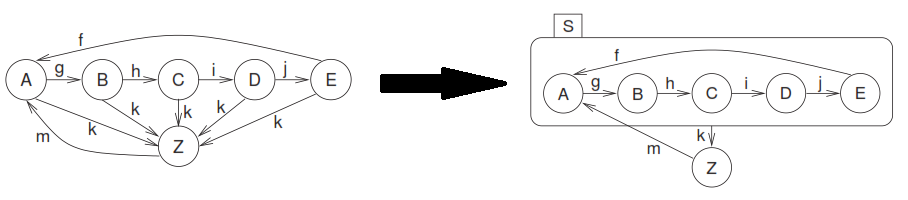
\includegraphics[width = 12cm]{images/FSM/Hierarchie}\\\\
Superzustand S beinhaltet die Zustände A, B, C, D und E. Angenommen, der Automat befindet sich in Zustand Z (wird auch als aktiver Zustand beschrieben). Wenn dann die Eingabe m am Automaten erfolgt, ist A der nächste Zustand. Wenn sich der Automat in Zustand S befindet und es gibt die Eingabe k, so ist Z der nächste Zustand, unabhängig davon, in welchem der Unterzustände A, B, C, D oder E sich der Automat tatsächlich befindet. In diesem Beispiel sind alle in S enthaltenen Zustände nicht-hierarchische Zustände. Im Allgemeinen könnten die Unterzustände von S selbst wieder Superzustände sein, die weitere Unterzustände enthalten.
\begin{itemize}
  \item Jeder Zustand, der nicht aus anderen Zuständen besteht, heisst Basiszustand.
  \item Superzustände S heissen ODER-Superzustände, wenn das System, das S enthält, sich zu jedem Zeitpunkt lediglich in einem einzigen Unterzustand von S befinden kann, solange es sich in S befindet.
\end{itemize}

\subsubsection{Modellierung von Hierarchie mit Default State (Standardzustand)}
\begin{multicols}{2}
Der Standardzustand kann in Superzuständen verwendet werden, um anzuzeigen, welcher der Unterzustände betreten wird, wenn der Superzustand betreten wird.
Dies wird mit einem kleinen ausgefüllten Kreis dargestellt.\\
\vfill\null
\columnbreak
\begin{center}
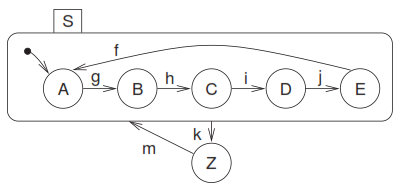
\includegraphics[width=0.6\linewidth]{images/FSM/Hierarchie_DefaultState}
\end{center}
\end{multicols}

\subsubsection{Modellierung von Hierarchie mit History}
Mit Hilfe des History-Mechanismus ist es möglich, in den letzten Unterzustand zurückzukehren, der aktiv war, bevor der Superzustand verlassen wurde. Der History-Mechanismus wird durch den Buchstaben H in
einem Kreis dargestellt.\\
\begin{minipage}[hbt]{8cm}
	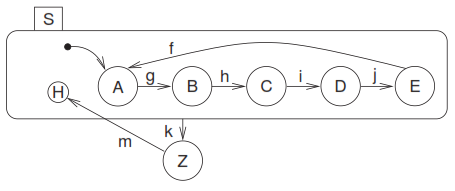
\includegraphics[width=6cm]{images/FSM/Hierarchie_History}
\end{minipage}
\begin{minipage}[hbt]{6cm}
	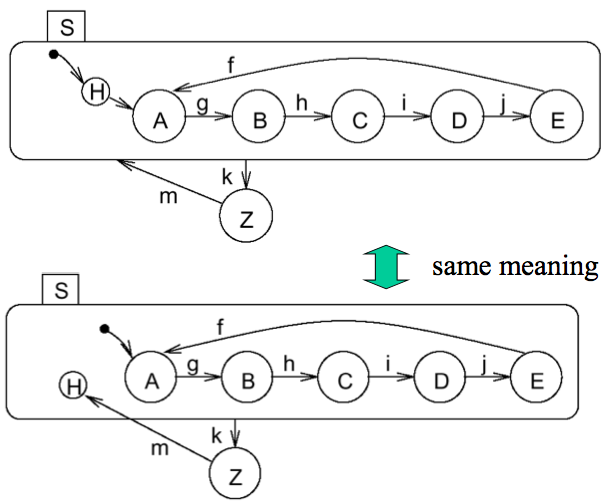
\includegraphics[width = 6cm]{images/FSM/history_default_state_mechanism}
\end{minipage}
\pagebreak\newpage

\subsubsection{Parallelität (UND-Superzustände)}
\begin{multicols}{2}
Eine Spezifikationstechnik muss auch in der Lage sein, Nebenläufigkeit und Parallelität darzustellen. Zu diesem Zweck gibt es eine zweite Art von Superzuständen, die sogenannten UND-Superzustände.
\begin{itemize}
\item Superzustände S heissen UND-Superzustände, wenn das System, das S enthält, sich in allen Unterzuständen von S gleichzeitig befindet,
solange es sich in S befindet.
\end{itemize}
\vfill\null
\columnbreak
\begin{center}
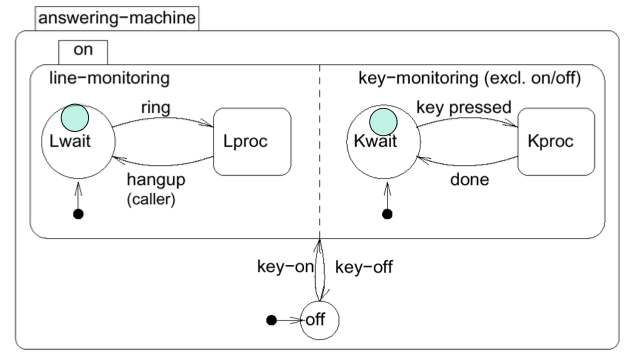
\includegraphics[width=0.8\linewidth]{images/FSM/AND_super_state}
\end{center}
\end{multicols}

\subsubsection{Zeitbedingungen}
\begin{multicols}{2}
Da es notwendig ist, in eingebetteten Systemen Zeitbedingungen zu modellieren, bieten Statecharts die sogenannten Timer an. Zeitbedingungen werden durch das gezackte Symbol dargestellt.\\
Wenn das System für die im Timer angegebene Zeitdauer im Timer-Zustand war, wird ein Time-Out ausgelöst und das System verlässt diesen Zustand. Timer können auch hierarchisch verwendet werden.\\
\vfill\null
\begin{center}
\columnbreak
Timer bei einem Telefon-Beantworter:\\
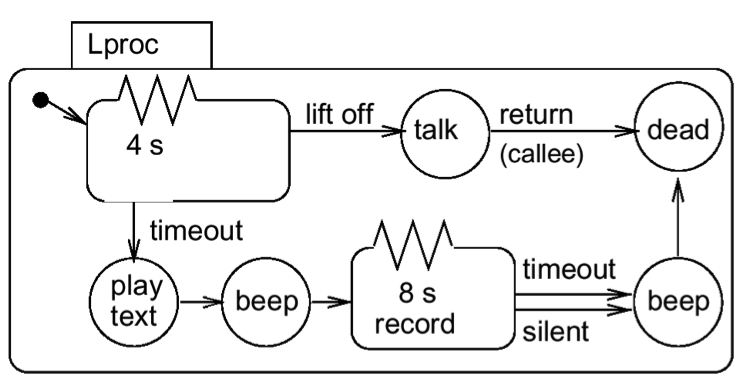
\includegraphics[width=8cm]{images/FSM/timer}
\end{center}
\end{multicols}
\newpage
